\documentclass{article}
\usepackage{a4wide}
\usepackage[utf8]{inputenc}
\usepackage{amsmath}
\usepackage{mathtools}
\usepackage{amssymb}
\usepackage[english]{babel}
\usepackage{mdframed}
\usepackage{systeme,}
\usepackage{lipsum}
\usepackage{relsize}
\usepackage{caption}
\usepackage{tikz}
\usepackage{tikz-3dplot}
\usepackage{pgfplots}
\usepackage{harpoon}%
\usepackage{graphicx}
\usepackage{wrapfig}
\usepackage{subcaption}
\usepackage{authblk}
\usepackage{float}
\usepackage{listings}
\usepackage{xcolor}
\usepackage{amsmath}
\usepackage{chngcntr}
\usepackage{amsthm}
\usepackage{comment}
\usepackage{commath}
\usepackage{hyperref}%Might remove, adds link to each reference
\usepackage{url}
\newcommand{\w}{\omega}
\newcommand{\curl}[1]{\mathbf{\nabla}\times \mathbf{#1}}
\newcommand{\grad}{\mathbf{\nabla}}
\newcommand{\dive}[1]{\mathbf{\nabla}\cdot \mathbf{#1}}
%\newcommand{\crr}{\mathfrak{r}}
\usepackage{calligra}

\DeclareMathAlphabet{\mathcalligra}{T1}{calligra}{m}{n}
\DeclareFontShape{T1}{calligra}{m}{n}{<->s*[2.2]callig15}{}
\newcommand{\crr}{\mathcalligra{r}\,}
\newcommand{\boldscriptr}{\pmb{\mathcalligra{r}}\,}
\newcommand{\res}[2]{\text{Res}(#1,#2)}

\title{Handin 2}
\author{Author : Andreas Evensen}
\date{Date: \today}
\definecolor{codegreen}{rgb}{0,0.6,0}
\definecolor{codegray}{rgb}{0.5,0.5,0.5}
\definecolor{codepurple}{rgb}{0.58,0,0.82}
\definecolor{backcolour}{rgb}{0.95,0.95,0.92}

\lstdefinestyle{mystyle}{
    backgroundcolor=\color{backcolour},   
    commentstyle=\color{codegreen},
    keywordstyle=\color{magenta},
    numberstyle=\tiny\color{codegray},
    stringstyle=\color{codepurple},
    basicstyle=\ttfamily\footnotesize,
    breakatwhitespace=false,         
    breaklines=true,                 
    captionpos=b,                    
    keepspaces=true,                 
    numbers=left,                    
    numbersep=5pt,                  
    showspaces=false,                
    showstringspaces=false,
    showtabs=false,                  
    tabsize=2
}

\lstset{style=mystyle}

\begin{document}

\maketitle

\section*{Problem 1}
Consider your space to be two-dimensional, such that $S_{i,j} = \frac{1}{2}(\partial_i u_j + \partial_j u_i)$ where $i,j = \{1,2\}$.
You can now define a two-dimensional Young's modulus $Y$ and a two-dimensional Poisson ratio $\sigma$. Find $Y$ and $\sigma$ as a function of the lame-coefficients $\lambda$ and $\mu$.
\subsection*{Answer}
Suppose a two-dimensional shape; this is valid for any shape:
\begin{figure}[H]
    \centering
    \begin{tikzpicture}[scale = 0.75]
        \draw (0,0) rectangle (5,5);
        %\draw[fill=red!10] (1, 1) circle (2pt);
        %\draw[fill=red!10] (1.2, 1.3) circle (2pt);
        %\draw[->, thin] (1, 1) -- (1.2, 1.3) node[below, right] {\small $\mathbf{u}(\Delta \mathbf{r})$};
        \draw[dashed] (0, 2.5) -- (5, 2.5) node[pos = 0.5, below] {$a$};
        \draw[->, color=blue!90] (5, 2.5) -- (6, 2.5) node[below] {$\sigma_{x,x}$};
        \draw[->, color=blue!90] (5, 5) -- (5, 6) node[right] {$\sigma_{y,x}$};
        \draw[->, color=blue!90] (0, 2.5) -- (-1, 2.5) node[below] {$\sigma_{x,x}$};
        \draw[->, color=blue!90] (0, 0) -- (0, -1) node[right] {$\sigma_{y,x}$};
        \draw[->, color=red!90] (2.5, 5) -- (2.5, 6) node[right] {$\sigma_{y,y}$};
        \draw[->, color=red!90] (5, 5) -- (6,5) node[right] {$\sigma_{x,y}$};
        \draw[->, color=red!90] (2.5, 0) -- (2.5, -1) node[right] {$\sigma_{y,y}$};
        \draw[->, color=red!90] (0, 0) -- (-1, 0) node[below] {$\sigma_{x,y}$};
    \end{tikzpicture}
    \caption{An arbitrary shape}
\end{figure}\noindent
The strain matrix is then defined as:
\begin{align*}
    S = \begin{pmatrix}
        \frac{\partial u_1}{\partial x_1} & \frac{1}{2}\left(\frac{\partial u_2}{\partial x_1} + \frac{\partial u_1}{\partial x_2}\right)\\
        \frac{1}{2}\left(\frac{\partial u_2}{\partial x_1} + \frac{\partial u_1}{\partial x_1}\right) & \frac{\partial u_2}{\partial x_2}
    \end{pmatrix}   
\end{align*}Assuming that the system is in mechanical equilibrium one has the following scenario:
\begin{align}
    \text{Net force}\quad & \sigma_{x,x} + \sigma_{x,y} = \sigma_{x,x} + \sigma_{x,y},\\
    \text{Net torque}\quad & a \cdot \left(\sigma_{x,y}-\sigma_{y,x}\right) = 0\implies \sigma_{x,y} = \sigma_{y,x}.\label{eq: torque-balance}
\end{align}Using equation \eqref{eq: torque-balance} one has $\sigma_{i,j} = \sigma_{j,i}$ where $(i,j)\in\{1,2\}$ which also relates that $\sigma$ is symmetric.
Imposing a small virtual deformation field yields a small work done on the particle in the solid:
\begin{align*}
    d W = - \sigma_{i,j}d S_{j,i}.
\end{align*}Taylor expanding Helmholtz free energy one obtains the following:
\begin{align*}
    F &= F_0 + A_{i,j,k,l}S_{i,j}S_{k,l},\\
    A_{i,j,k,l}S_{i,j}S_{k,l} &= \frac{\lambda}{2} S_{i,i}\cdot S_{j,j} + \mu \cdot S_{i,j}\cdot S_{i,j}\\
    \implies F &= F_0 + \frac{\lambda}{2} S_{i,i}\cdot S_{j,j} + \mu \cdot S_{i,j}\cdot S_{i,j} + \text{h.o.t} 
\end{align*}Furthermore, one can rewrite $S_{i,j}$ in terms of the following:
\begin{align*}
    S_{i,j} &= (S_{i,j} - \frac{1}{2}\delta_{i,j}S_{k,k}) + \frac{1}{2}\delta_{i,j}S_{k,k},
\end{align*}where one has split out the sheer stress and pure compression/extension in a two-dimensional plane. 
One can thus write down the following:
\begin{align*}
    \tilde{F} &= \frac{\lambda}{2}\left(S_{i,j} - \frac{1}{2}\delta_{i,j}S_{k,k}\right)^2 + \mu\left(\frac{1}{2}\delta_{i,j}S_{k,k}\right)^2\\
    d\tilde{F} &= \mu \delta_{i,j}S_{k,k}dS_{k,k} + \lambda\left(S_{i,j} - \frac{1}{2}\delta_{i,j}S_{k,k}\right)d\left(S_{i,j} - \frac{1}{2}\delta_{i,j}S_{k,k}\right).
\end{align*}
The stress tensor is given by the following expression:
\begin{align}
    \sigma_{i,j} &= \frac{\partial F}{\partial S_{i,j}}\Bigg|_T\label{eq: sigma}\\
    &= \mu \delta_{i,j}S_{k,k}  + \lambda \left(S_{i,j} - \frac{1}{2}\delta_{i,j}S_{k,k}\right).\nonumber
\end{align}From equation \eqref{eq: sigma} one finds that the Young's modulus and Poisson ratio, in terms of Lamé's coefficients, is given by:
\begin{align*}
    Y &= \frac{4\mu(\lambda + \mu)}{\lambda + 2\mu},\\
    \sigma &= \frac{\lambda}{\lambda + 2\mu}.
\end{align*}

\begin{comment}
Since this is linear in $S$ one can invert the system which can be done in the following manner:
\begin{align*}
    \begin{pmatrix}
        \sigma_{1,1}&\sigma_{1,2}\\
        \sigma_{2,1}&\sigma_{2,2}
    \end{pmatrix} &= \mu \begin{pmatrix}
        S_{11}&0\\
        0&S_{2,2}
    \end{pmatrix} + \lambda \begin{pmatrix}
        \frac{S_{1,1}}{2}&S_{1,2}\\
        S_{2,1}&\frac{S_{2,2}}{2}
    \end{pmatrix}\\
    &=\left(\begin{pmatrix}
        \mu&0\\
        0&\mu
    \end{pmatrix} +\begin{pmatrix}
        \frac{\lambda}{2}& 1\\
        1&\frac{\lambda}{2}
    \end{pmatrix}\right)S\\
    &= \begin{pmatrix}
        \mu\frac{\lambda}{2}&\lambda\\
        \lambda&\mu\frac{\lambda}{2}
    \end{pmatrix}S\\
    \implies S &= \begin{pmatrix}
        \mu\frac{\lambda}{2}&\lambda\\
        \lambda&\mu\frac{\lambda}{2}
    \end{pmatrix}^{-1}\sigma\\
    &=\frac{2}{\lambda(\mu^2-4)}\begin{pmatrix}
        \mu&-2\\
        -2&\mu
    \end{pmatrix}\begin{pmatrix}
        \sigma_{1,1}&\sigma_{1,2}\\
        \sigma_{2,1}&\sigma_{2,2}
    \end{pmatrix}
\end{align*}The Poisson ratio is found in the first term of $S$;
\end{comment}

\section*{Problem 2}
Consider a rod of length $l$ rotating with an angular velocity $\w$ about an axis perpendicular to the rod.
The rod has a mass-density $\varrho$, Young's modulus $Y$  and Poisson's ratio $\sigma$. Calculate the deformation.
\begin{figure}[H]
    \centering
    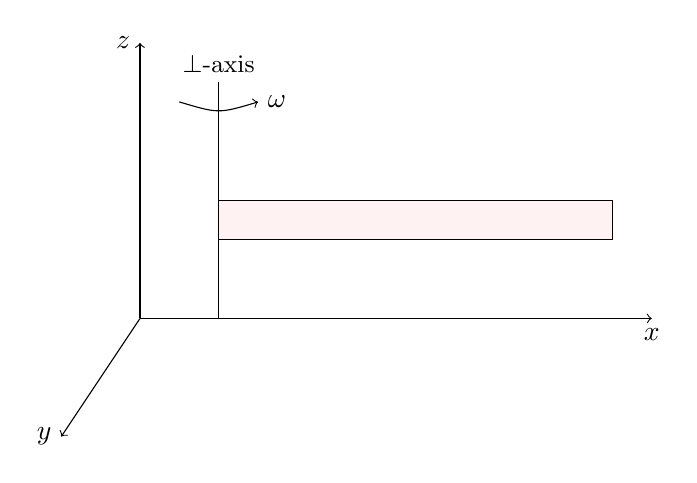
\begin{tikzpicture}
        \draw[fill=red!5] (0,0) rectangle (5,0.5);
        \draw (0, -1) -- (0,2) node[above] {\small$\perp$-axis};
        \draw[->] (-0.5, 1.75) .. controls (0, 1.6) .. (0.5, 1.75) node[right] {$\w$};
        \draw[->] (-1, -1) -- (5.5, -1) node[below] {$x$};
        \draw[->] (-1, -1) -- (-1, 2.5) node[left] {$z$};
        \draw[->] (-1, -1) -- (-2, -2.5) node[left] {$y$};
    \end{tikzpicture}
    \caption{Figure of the system}
\end{figure}
\subsection*{Answer}
Using the coordinate system as shown above one can see that the rotation is about the $z$ axis, and thus the force exhibited is in the $x-y$-plane; which one can express in cylindrical coordinate as $\rho$.
\begin{comment}
\begin{align*}
    \bar{\nabla}\left(\text{div}~\mathbf{u}\right) &= -\varrho\w^2 \cdot \frac{(\rho^2 - l^2)}{2Y}\\
\end{align*}
This is then the solution for a rod rotating around an axis perpendicular to the rod, since its only dependent on the distance from the axis of rotation, $\rho$.
\end{comment}
\begin{align*}
    \omega_{\rho, \rho} = \varrho\w^2\frac{\rho^2}{2} +c(\rho, z).
\end{align*}From boundary conditions one can see that $c_1 = - \varrho\w^2\frac{L^2}{2}$. From this, one get that the strain-element is given by:
\begin{align*}
    S_{\rho,\rho} &= \frac{\varrho\w^2}{2Y}(\rho^2 - L^2)\\
    u_\rho(\rho) &= \int_0^\rho\frac{\varrho\w^2}{2Y}(\tilde{\rho}^2 - L^2)d\tilde{\rho}\\
    &= \frac{\varrho\w^2}{2Y}\left(\frac{\rho^3}{3} - L^2\rho\right)\\
\end{align*}
\section*{Problem 3}
Determine the deformation of a solid sphere of radius $r$, mass-density $\rho$, Young's modulus $Y$ and Poisson ratio $\sigma$ under the action of its own gravity.
\begin{figure}[H]
    \centering
    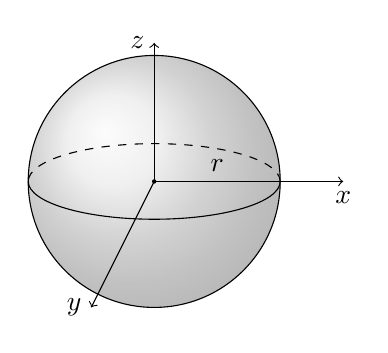
\begin{tikzpicture}[scale = 0.8]
        \shade[ball color = gray!40, opacity = 0.4] (0, 0) circle (2cm);
        \draw (0, 0) circle (2cm);
        \draw (-2, 0) arc (180:360:2 and 0.6);
        \draw[dashed] (2, 0) arc (0:180:2 and 0.6);
        \fill[fill=black] (0, 0) circle (1pt);
        \draw[dashed] (0, 0) -- node[above]{$r$} (2, 0);
        \draw[->] (0,0) -- (3,0) node[below] {$x$};
        \draw[->] (0,0) -- (0,2.2) node[left] {$z$};
        \draw[->] (0,0) -- (-1,-2) node[left] {$y$};
    \end{tikzpicture}
    \caption{Sketch of the system}
\end{figure}
\subsection*{Answer}
Due to the gravity of the sphere, pressure will increase closer to the center of the sphere. This will cause the sphere to deform, and the deformation will be dependent on the distance from the center of the sphere.
Since a sphere is spherically symmetric, one can use spherical coordinates to describe the deformation, and the deformation is only dependent on the radial component; the other component might not be non-zero, but they will cancel each-other.
We can then use the following equation:
\begin{align*}
    \frac{1}{r^2}\frac{d}{dr}\left[r^2\frac{du}{dr}\right] &= \frac{G\rho r}{R}\cdot\frac{(1+\sigma)(1-2\sigma)}{Y(1-\sigma)}\\
    \frac{d}{dr}\left[r^2\frac{du}{dr}\right] &= G\rho\frac{r^3}{R}\frac{(1+\sigma)(1-2\sigma)}{Y(1-\sigma)}\\
    \left[r^2\frac{du}{dr}\right] &= G\rho\frac{r^4}{4R}\frac{(1+\sigma)(1-2\sigma)}{Y(1-\sigma)}+ A\\
    \frac{du}{dr} &= G\rho\frac{r^2}{4R}\frac{(1+\sigma)(1-2\sigma)}{Y(1-\sigma)} + \frac{A}{r^2}\\
    u(r) &= G\rho\frac{r^3}{12R}\frac{(1+\sigma)(1-2\sigma)}{Y(1-\sigma)} - \frac{A}{r}\\
\end{align*}where $G$ is the gravitational constant.

\end{document}
 